% Created by tikzDevice version 0.9 on 2016-01-25 21:21:54
% !TEX encoding = UTF-8 Unicode
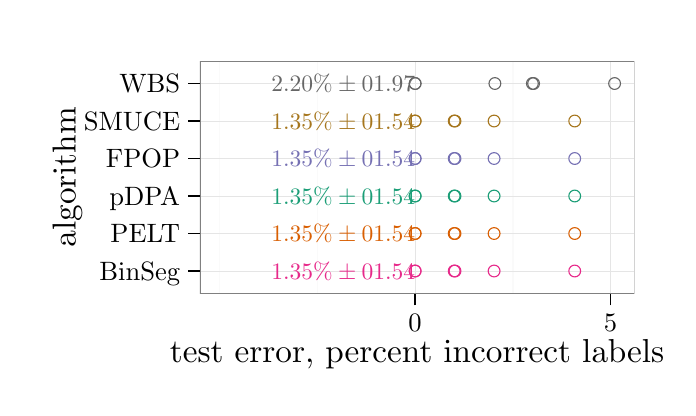
\begin{tikzpicture}[x=1pt,y=1pt]
\definecolor{fillColor}{RGB}{255,255,255}
\path[use as bounding box,fill=fillColor,fill opacity=0.00] (0,0) rectangle (231.26,130.09);
\begin{scope}
\path[clip] (  0.00,  0.00) rectangle (231.26,130.09);
\definecolor{drawColor}{RGB}{255,255,255}
\definecolor{fillColor}{RGB}{255,255,255}

\path[draw=drawColor,line width= 0.6pt,line join=round,line cap=round,fill=fillColor] (  0.00, -0.00) rectangle (231.26,130.09);
\end{scope}
\begin{scope}
\path[clip] ( 62.21, 34.03) rectangle (219.22,118.04);
\definecolor{fillColor}{RGB}{255,255,255}

\path[fill=fillColor] ( 62.21, 34.03) rectangle (219.22,118.04);
\definecolor{drawColor}{gray}{0.98}

\path[draw=drawColor,line width= 0.6pt,line join=round] ( 69.35, 34.03) --
	( 69.35,118.04);

\path[draw=drawColor,line width= 0.6pt,line join=round] (104.67, 34.03) --
	(104.67,118.04);

\path[draw=drawColor,line width= 0.6pt,line join=round] (175.32, 34.03) --
	(175.32,118.04);
\definecolor{drawColor}{gray}{0.90}

\path[draw=drawColor,line width= 0.2pt,line join=round] ( 62.21, 42.16) --
	(219.22, 42.16);

\path[draw=drawColor,line width= 0.2pt,line join=round] ( 62.21, 55.71) --
	(219.22, 55.71);

\path[draw=drawColor,line width= 0.2pt,line join=round] ( 62.21, 69.26) --
	(219.22, 69.26);

\path[draw=drawColor,line width= 0.2pt,line join=round] ( 62.21, 82.81) --
	(219.22, 82.81);

\path[draw=drawColor,line width= 0.2pt,line join=round] ( 62.21, 96.36) --
	(219.22, 96.36);

\path[draw=drawColor,line width= 0.2pt,line join=round] ( 62.21,109.91) --
	(219.22,109.91);

\path[draw=drawColor,line width= 0.2pt,line join=round] (140.00, 34.03) --
	(140.00,118.04);

\path[draw=drawColor,line width= 0.2pt,line join=round] (210.64, 34.03) --
	(210.64,118.04);
\definecolor{drawColor}{RGB}{231,41,138}

\node[text=drawColor,anchor=base east,inner sep=0pt, outer sep=0pt, scale=  0.85] at (140.00, 39.24) {$1.35\% \pm 01.54$};
\definecolor{drawColor}{RGB}{217,95,2}

\node[text=drawColor,anchor=base east,inner sep=0pt, outer sep=0pt, scale=  0.85] at (140.00, 52.79) {$1.35\% \pm 01.54$};
\definecolor{drawColor}{RGB}{27,158,119}

\node[text=drawColor,anchor=base east,inner sep=0pt, outer sep=0pt, scale=  0.85] at (140.00, 66.33) {$1.35\% \pm 01.54$};
\definecolor{drawColor}{RGB}{117,112,179}

\node[text=drawColor,anchor=base east,inner sep=0pt, outer sep=0pt, scale=  0.85] at (140.00, 79.88) {$1.35\% \pm 01.54$};
\definecolor{drawColor}{RGB}{166,118,29}

\node[text=drawColor,anchor=base east,inner sep=0pt, outer sep=0pt, scale=  0.85] at (140.00, 93.43) {$1.35\% \pm 01.54$};
\definecolor{drawColor}{gray}{0.40}

\node[text=drawColor,anchor=base east,inner sep=0pt, outer sep=0pt, scale=  0.85] at (140.00,106.98) {$2.20\% \pm 01.97$};
\definecolor{drawColor}{RGB}{231,41,138}

\path[draw=drawColor,line width= 0.4pt,line join=round,line cap=round] (154.41, 42.16) circle (  2.13);

\path[draw=drawColor,line width= 0.4pt,line join=round,line cap=round] (140.00, 42.16) circle (  2.13);

\path[draw=drawColor,line width= 0.4pt,line join=round,line cap=round] (140.00, 42.16) circle (  2.13);

\path[draw=drawColor,line width= 0.4pt,line join=round,line cap=round] (154.12, 42.16) circle (  2.13);

\path[draw=drawColor,line width= 0.4pt,line join=round,line cap=round] (168.54, 42.16) circle (  2.13);

\path[draw=drawColor,line width= 0.4pt,line join=round,line cap=round] (197.67, 42.16) circle (  2.13);
\definecolor{drawColor}{RGB}{217,95,2}

\path[draw=drawColor,line width= 0.4pt,line join=round,line cap=round] (154.41, 55.71) circle (  2.13);

\path[draw=drawColor,line width= 0.4pt,line join=round,line cap=round] (140.00, 55.71) circle (  2.13);

\path[draw=drawColor,line width= 0.4pt,line join=round,line cap=round] (140.00, 55.71) circle (  2.13);

\path[draw=drawColor,line width= 0.4pt,line join=round,line cap=round] (154.12, 55.71) circle (  2.13);

\path[draw=drawColor,line width= 0.4pt,line join=round,line cap=round] (168.54, 55.71) circle (  2.13);

\path[draw=drawColor,line width= 0.4pt,line join=round,line cap=round] (197.67, 55.71) circle (  2.13);
\definecolor{drawColor}{RGB}{27,158,119}

\path[draw=drawColor,line width= 0.4pt,line join=round,line cap=round] (154.41, 69.26) circle (  2.13);

\path[draw=drawColor,line width= 0.4pt,line join=round,line cap=round] (140.00, 69.26) circle (  2.13);

\path[draw=drawColor,line width= 0.4pt,line join=round,line cap=round] (140.00, 69.26) circle (  2.13);

\path[draw=drawColor,line width= 0.4pt,line join=round,line cap=round] (154.12, 69.26) circle (  2.13);

\path[draw=drawColor,line width= 0.4pt,line join=round,line cap=round] (168.54, 69.26) circle (  2.13);

\path[draw=drawColor,line width= 0.4pt,line join=round,line cap=round] (197.67, 69.26) circle (  2.13);
\definecolor{drawColor}{RGB}{117,112,179}

\path[draw=drawColor,line width= 0.4pt,line join=round,line cap=round] (154.41, 82.81) circle (  2.13);

\path[draw=drawColor,line width= 0.4pt,line join=round,line cap=round] (140.00, 82.81) circle (  2.13);

\path[draw=drawColor,line width= 0.4pt,line join=round,line cap=round] (140.00, 82.81) circle (  2.13);

\path[draw=drawColor,line width= 0.4pt,line join=round,line cap=round] (154.12, 82.81) circle (  2.13);

\path[draw=drawColor,line width= 0.4pt,line join=round,line cap=round] (168.54, 82.81) circle (  2.13);

\path[draw=drawColor,line width= 0.4pt,line join=round,line cap=round] (197.67, 82.81) circle (  2.13);
\definecolor{drawColor}{RGB}{166,118,29}

\path[draw=drawColor,line width= 0.4pt,line join=round,line cap=round] (154.41, 96.36) circle (  2.13);

\path[draw=drawColor,line width= 0.4pt,line join=round,line cap=round] (140.00, 96.36) circle (  2.13);

\path[draw=drawColor,line width= 0.4pt,line join=round,line cap=round] (140.00, 96.36) circle (  2.13);

\path[draw=drawColor,line width= 0.4pt,line join=round,line cap=round] (154.12, 96.36) circle (  2.13);

\path[draw=drawColor,line width= 0.4pt,line join=round,line cap=round] (168.54, 96.36) circle (  2.13);

\path[draw=drawColor,line width= 0.4pt,line join=round,line cap=round] (197.67, 96.36) circle (  2.13);
\definecolor{drawColor}{gray}{0.40}

\path[draw=drawColor,line width= 0.4pt,line join=round,line cap=round] (168.83,109.91) circle (  2.13);

\path[draw=drawColor,line width= 0.4pt,line join=round,line cap=round] (140.00,109.91) circle (  2.13);

\path[draw=drawColor,line width= 0.4pt,line join=round,line cap=round] (140.00,109.91) circle (  2.13);

\path[draw=drawColor,line width= 0.4pt,line join=round,line cap=round] (182.38,109.91) circle (  2.13);

\path[draw=drawColor,line width= 0.4pt,line join=round,line cap=round] (182.81,109.91) circle (  2.13);

\path[draw=drawColor,line width= 0.4pt,line join=round,line cap=round] (212.08,109.91) circle (  2.13);
\definecolor{drawColor}{gray}{0.50}

\path[draw=drawColor,line width= 0.6pt,line join=round,line cap=round] ( 62.21, 34.03) rectangle (219.22,118.04);
\end{scope}
\begin{scope}
\path[clip] (  0.00,  0.00) rectangle (231.26,130.09);
\definecolor{drawColor}{RGB}{0,0,0}

\node[text=drawColor,anchor=base east,inner sep=0pt, outer sep=0pt, scale=  0.96] at ( 55.10, 38.86) {BinSeg};

\node[text=drawColor,anchor=base east,inner sep=0pt, outer sep=0pt, scale=  0.96] at ( 55.10, 52.41) {PELT};

\node[text=drawColor,anchor=base east,inner sep=0pt, outer sep=0pt, scale=  0.96] at ( 55.10, 65.96) {pDPA};

\node[text=drawColor,anchor=base east,inner sep=0pt, outer sep=0pt, scale=  0.96] at ( 55.10, 79.51) {FPOP};

\node[text=drawColor,anchor=base east,inner sep=0pt, outer sep=0pt, scale=  0.96] at ( 55.10, 93.06) {SMUCE};

\node[text=drawColor,anchor=base east,inner sep=0pt, outer sep=0pt, scale=  0.96] at ( 55.10,106.61) {WBS};
\end{scope}
\begin{scope}
\path[clip] (  0.00,  0.00) rectangle (231.26,130.09);
\definecolor{drawColor}{RGB}{0,0,0}

\path[draw=drawColor,line width= 0.6pt,line join=round] ( 57.95, 42.16) --
	( 62.21, 42.16);

\path[draw=drawColor,line width= 0.6pt,line join=round] ( 57.95, 55.71) --
	( 62.21, 55.71);

\path[draw=drawColor,line width= 0.6pt,line join=round] ( 57.95, 69.26) --
	( 62.21, 69.26);

\path[draw=drawColor,line width= 0.6pt,line join=round] ( 57.95, 82.81) --
	( 62.21, 82.81);

\path[draw=drawColor,line width= 0.6pt,line join=round] ( 57.95, 96.36) --
	( 62.21, 96.36);

\path[draw=drawColor,line width= 0.6pt,line join=round] ( 57.95,109.91) --
	( 62.21,109.91);
\end{scope}
\begin{scope}
\path[clip] (  0.00,  0.00) rectangle (231.26,130.09);
\definecolor{drawColor}{RGB}{0,0,0}

\path[draw=drawColor,line width= 0.6pt,line join=round] (140.00, 29.77) --
	(140.00, 34.03);

\path[draw=drawColor,line width= 0.6pt,line join=round] (210.64, 29.77) --
	(210.64, 34.03);
\end{scope}
\begin{scope}
\path[clip] (  0.00,  0.00) rectangle (231.26,130.09);
\definecolor{drawColor}{RGB}{0,0,0}

\node[text=drawColor,anchor=base,inner sep=0pt, outer sep=0pt, scale=  0.96] at (140.00, 20.31) {0};

\node[text=drawColor,anchor=base,inner sep=0pt, outer sep=0pt, scale=  0.96] at (210.64, 20.31) {5};
\end{scope}
\begin{scope}
\path[clip] (  0.00,  0.00) rectangle (231.26,130.09);
\definecolor{drawColor}{RGB}{0,0,0}

\node[text=drawColor,anchor=base,inner sep=0pt, outer sep=0pt, scale=  1.20] at (140.72,  9.03) {test error, percent incorrect labels};
\end{scope}
\begin{scope}
\path[clip] (  0.00,  0.00) rectangle (231.26,130.09);
\definecolor{drawColor}{RGB}{0,0,0}

\node[text=drawColor,rotate= 90.00,anchor=base,inner sep=0pt, outer sep=0pt, scale=  1.20] at ( 17.30, 76.04) {algorithm};
\end{scope}
\end{tikzpicture}
